\chapter{The ATLAS Experiment at the LHC}
\label{ch:detector}
\epigraph{\emph{We are rather like children, who must take a watch to pieces to see how it works.}}{Sir Ernest Rutherford}

	\ac{ATLAS} (A Toroidal LHC ApparatuS) is one of the four main experiments\footnote{\ac{ATLAS}, \ac{CMS}, \ac{ALICE}, \ac{LHCb}} taking data at a centre-of-mass energy of $13$ TeV using beams delivered by the \ac{LHC}. In this chapter an overview of the \ac{LHC} will be given in Section~\ref{sec:lhc}, then the \ac{ATLAS} detector will be described in Section~\ref{sec:det}, and finally the Trigger system, used to cleverly select the data, will be described in Section~\ref{sec:trigSyst}. A more in-depth description of the Trigger algorithms the author has been involved in will be given in Chapter~\ref{ch:trigger}.


	% --------------------------------
	% -------  THE LHC
	% --------------------------------
	\section{The LHC}
	\label{sec:lhc}
	
		As of today, the \ac{LHC}~\cite{LHCDesignReport} is the world’s largest and most powerful particle accelerator. It was designed to help answer some of the fundamental open questions in particle physics by colliding protons at an unprecedented energy and luminosity. It is located at \ac{CERN}, in the Geneva area, at a depth ranging from 50 to 175 metres underground. It consists of a 27-kilometre ring made of superconducting magnets, and inside it two high-energy particle beams travel in opposite directions and in separate beam pipes. 

		The beams are guided around the ring by a strong magnetic field generated by coils - made of special electric cables - that can operate in a superconducting regime. A total of 1232 superconducting dipole and 392 quadrupole magnets, with an average magnetic field of 8.3 T, are employed and kept at a temperature below 1.7 K, in order to preserve their superconducting properties. The former are used to bend the beams and the latter to keep them focused while they get accelerated. 
		%In order for this to be possible though, the magnets have to remain at a temperature of -271.3$^\circ$C for which a distribution system of liquid helium is employed.
		
		The collider first went live on September 2008 even though, due to a magnet quench incident that damaged over 50 superconducting magnets, it has been fully operational since November 2009 when low-energy beams circulated in the tunnel for the first time since the incident. This also marked the start of the main research programme and the beginning of the so-called Run 1: first operational run (2009 - 2013).


		\subsection*{Performance of the LHC}

			In June 2015 the \ac{LHC} restarted delivering physics data, after a two-year upgrade programme, the so-called \ac{LS1}, during which the magnets were upgraded to handle the current required to circulate 7-TeV beams. It was the beginning of the so-called Run 2 - second operational run (2015-2018) - during which the \ac{LHC} has collided up to $10^{11}$ bunches of protons every 25 ns at the design luminosity\footnote{the highest luminosity the detector was designed to cope with} of $2 \cdot 10^{34} \mathrm{cm}^{-2}\mathrm{s}^{-1}$. The definition of the luminosity is:

			\begin{equation}
				{\mathcal L} = f \frac{n_b N_1 N_2}{4 \pi \sigma_x \sigma_y}
			\label{eq:lumi}
			\end{equation}

			\noindent where $N_1$ and $N_2$ are the number of protons per bunch in each of the colliding beams, $f$ is the revolution frequency of the bunch collisions, $n_b$ the number of proton per bunch, and $\sigma_x$ and $\sigma_y$ are the horizontal and vertical dimensions of the beam. The luminosity is strictly related to the number of collisions occurring during a certain experiment via the following: 

			\begin{equation}
					{\mathcal N}_{\mathrm{event}} = {\mathcal L} \sigma_{\mathrm{event}}
			\label{eq:lumiEvt}
			\end{equation}

			\noindent where $\sigma_{\mathrm{event}}$ is the cross section of the process under investigation.  It has not only collided protons but also heavy ions, in particular lead nuclei at $\sqrt{s_{NN}} = 5.02$ TeV, at a luminosity of $10^{27} \mathrm{cm}^{-2} \mathrm{s}^{-1}$\cite{HI2015}.



		\subsection*{Acceleration stages}

			\begin{figure}[!htb]
				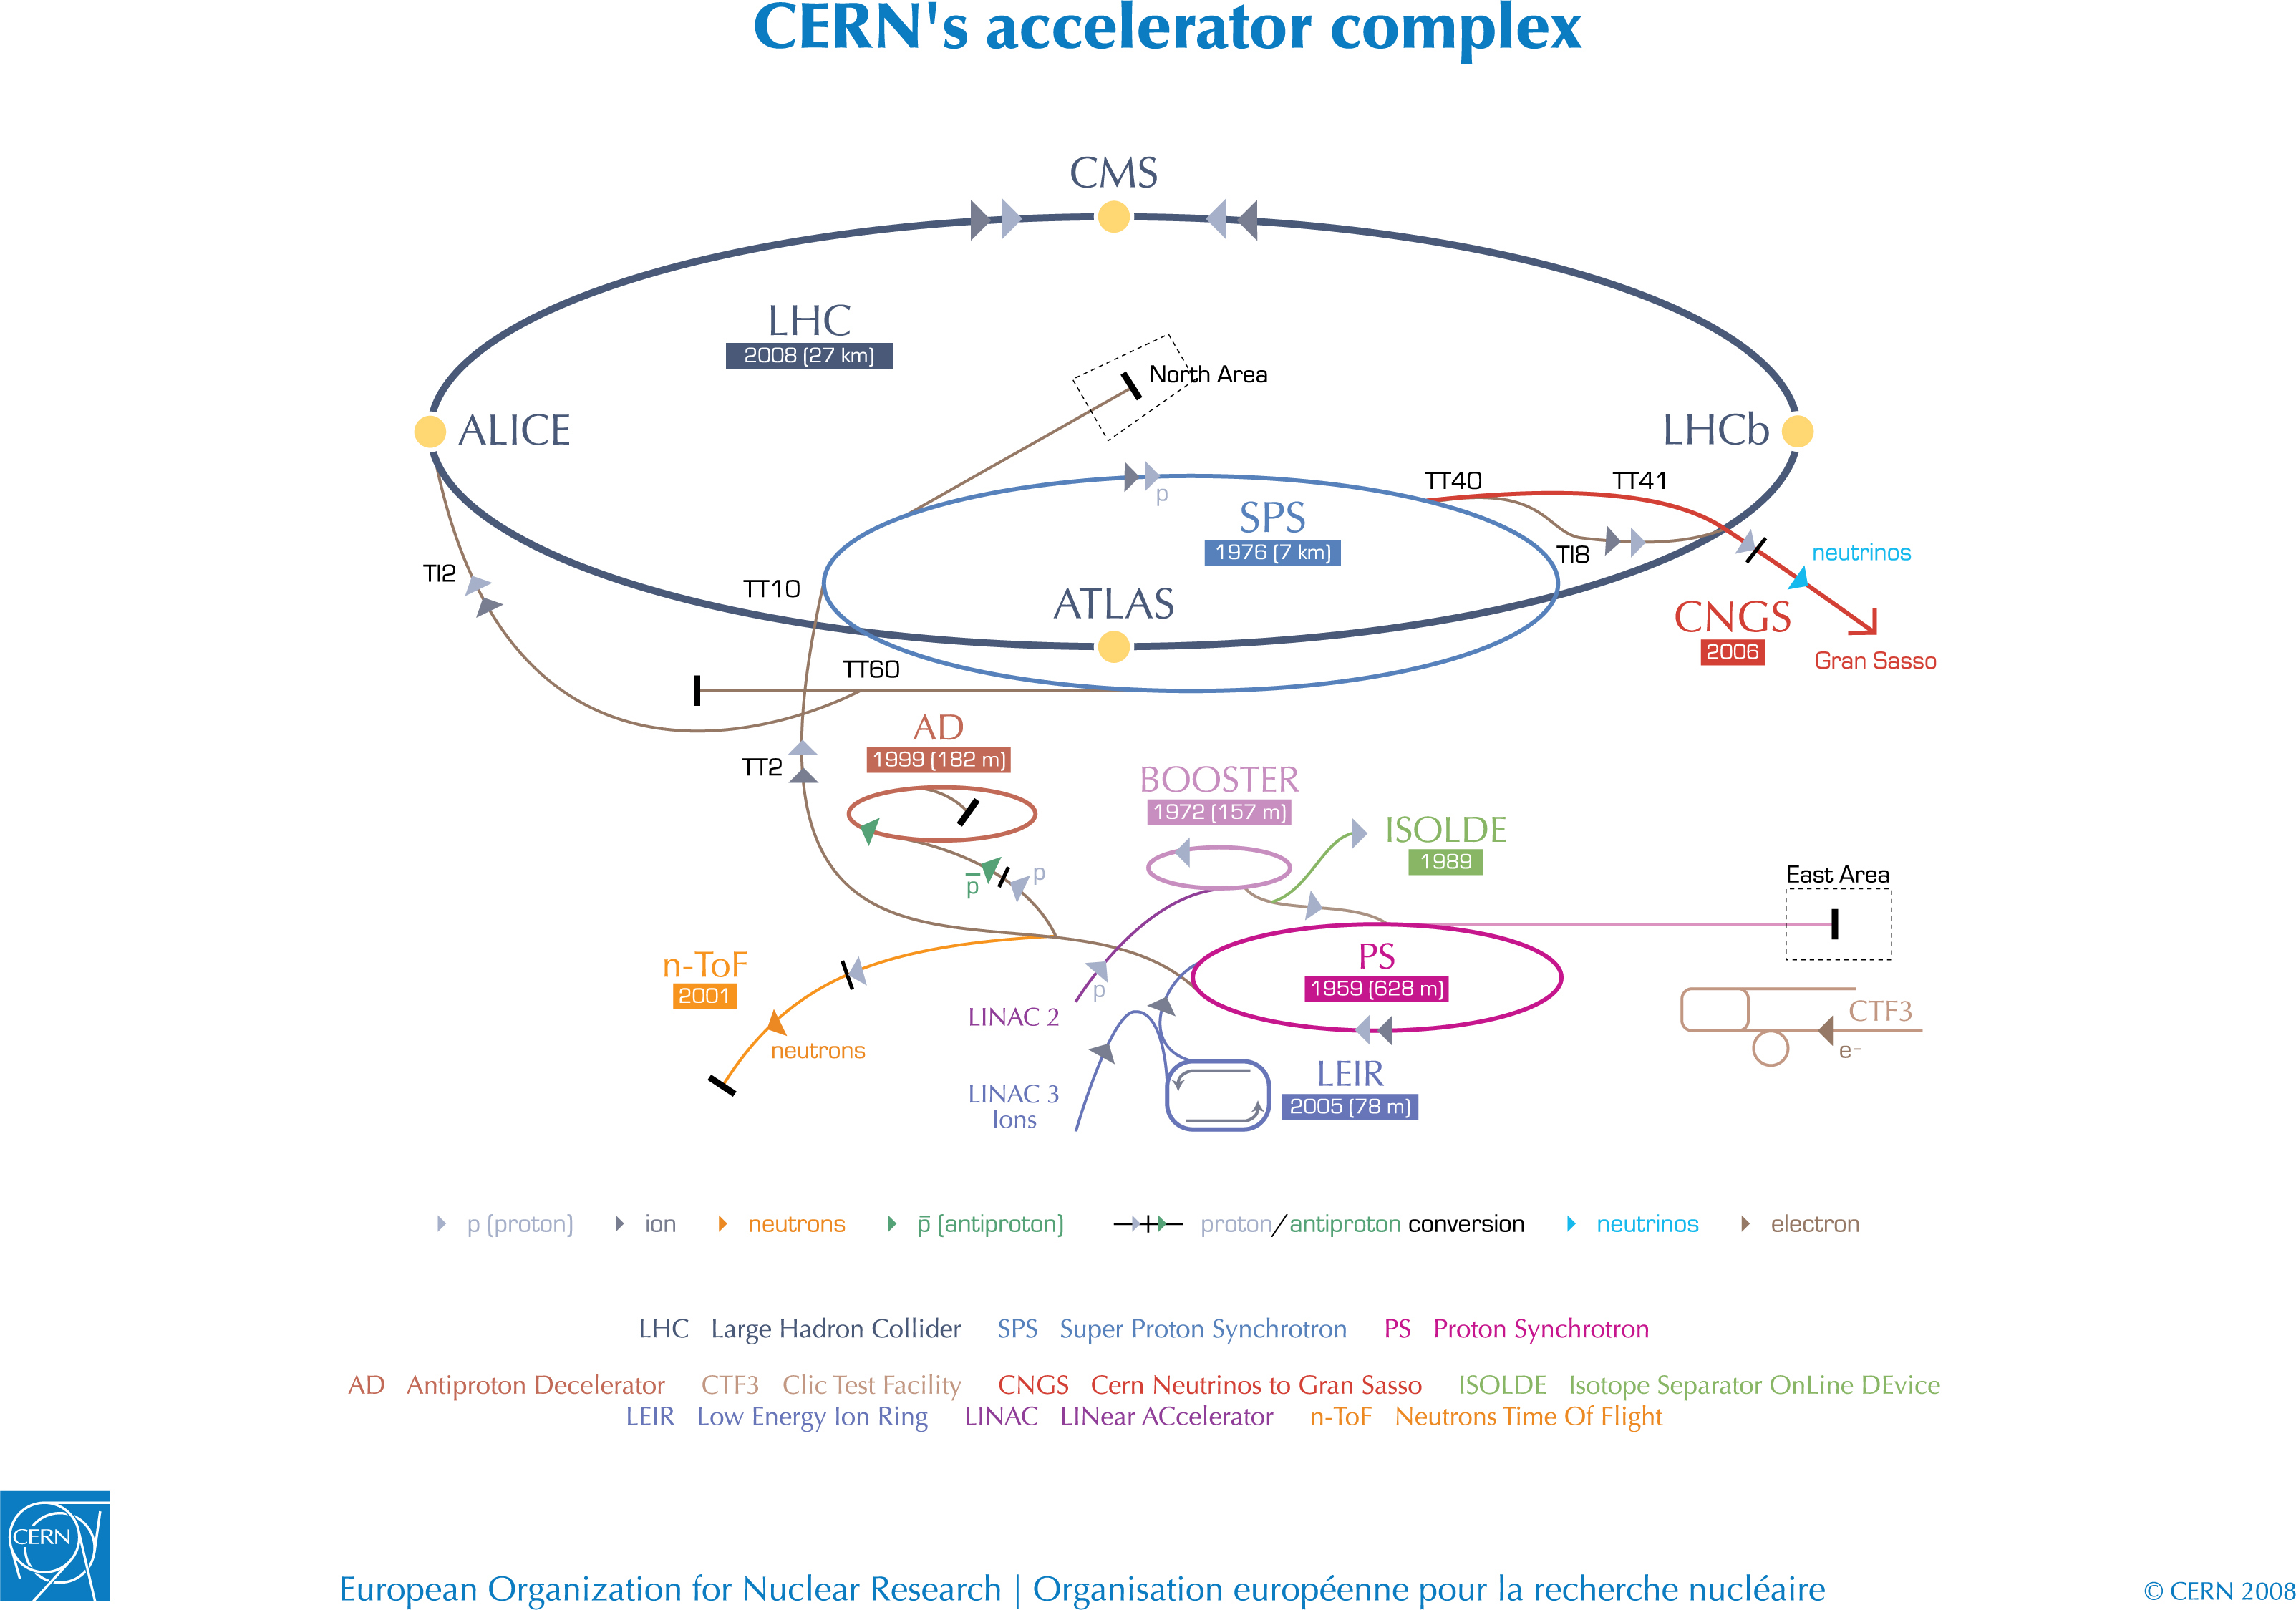
\includegraphics[width=\textwidth]{Detector/cern-acc-complex.jpg}
				\caption{\ac{CERN} Accelerator complex. The \ac{LHC} is the last ring (dark grey line). Smaller machines are used for early-stage acceleration and also to provide beams for other experiments~\cite{Lefevre2008}.}
				\label{fig:cern-acc-complex}
			\end{figure}

			Before reaching the maximum energy, the proton beams are accelerated by smaller accelerators through various stages. Figure~\ref{fig:cern-acc-complex} shows a sketch of the \ac{CERN}'s accelerator complex. It all begins with the \ac{LINAC2}. Here protons are accelerated up to 50 MeV, and then injected in the \ac{PSB} where they reach 1.4 \GeV. The next stage is the Proton Synchrotron, which boosts the beams up to 25 \GeV\, and then \ac{SPS} makes them reach energies up to 450 \GeV. Eventually, the beams are injected in bunches with a 25 ns spacing into the \ac{LHC}, where they travel in opposite directions, while they are accelerated to up to a centre-of-mass energy of 13 TeV. Once the bunches reach the maximum energy, they are made collide at four different points, inside four experiments around the ring~\cite{LHCDesignReport}. 

			The heavy ion beams acceleration procedure is slightly different. Their journey starts at \ac{LINAC3}, and the \ac{LEIR} then, before they make their way into the Proton Synchrotron where they follow the same path as the protons. 

			The four large detectors on the collision points are; the multi-purpose detectors \ac{ATLAS}~\cite{ATLASJINST}, and \ac{CMS}~\cite{CMSJINST}, \ac{LHCb}~\cite{LHCb2008}, which focuses on flavour physics, and \ac{ALICE}~\cite{ALICEJINST} which specialises in heavy ion physics. The \emph{big four} are not the only experiments at the \ac{CERN}'s accelerator complex. There also are smaller experiments based at the the four caverns about the collision points e.g. \ac{TOTEM}~\cite{1748-0221-3-08-S08007}, \ac{LHCf}~\cite{Adriani:926196} and \ac{MoEDAL}~\cite{Pinfold:2017dot}, but these will not be discussed any further.
		


	% --------------------------------
	% -------  THE DETECTOR
	% --------------------------------
	\section{The ATLAS Detector}
	\label{sec:det}

		\begin{figure}[!htb]
			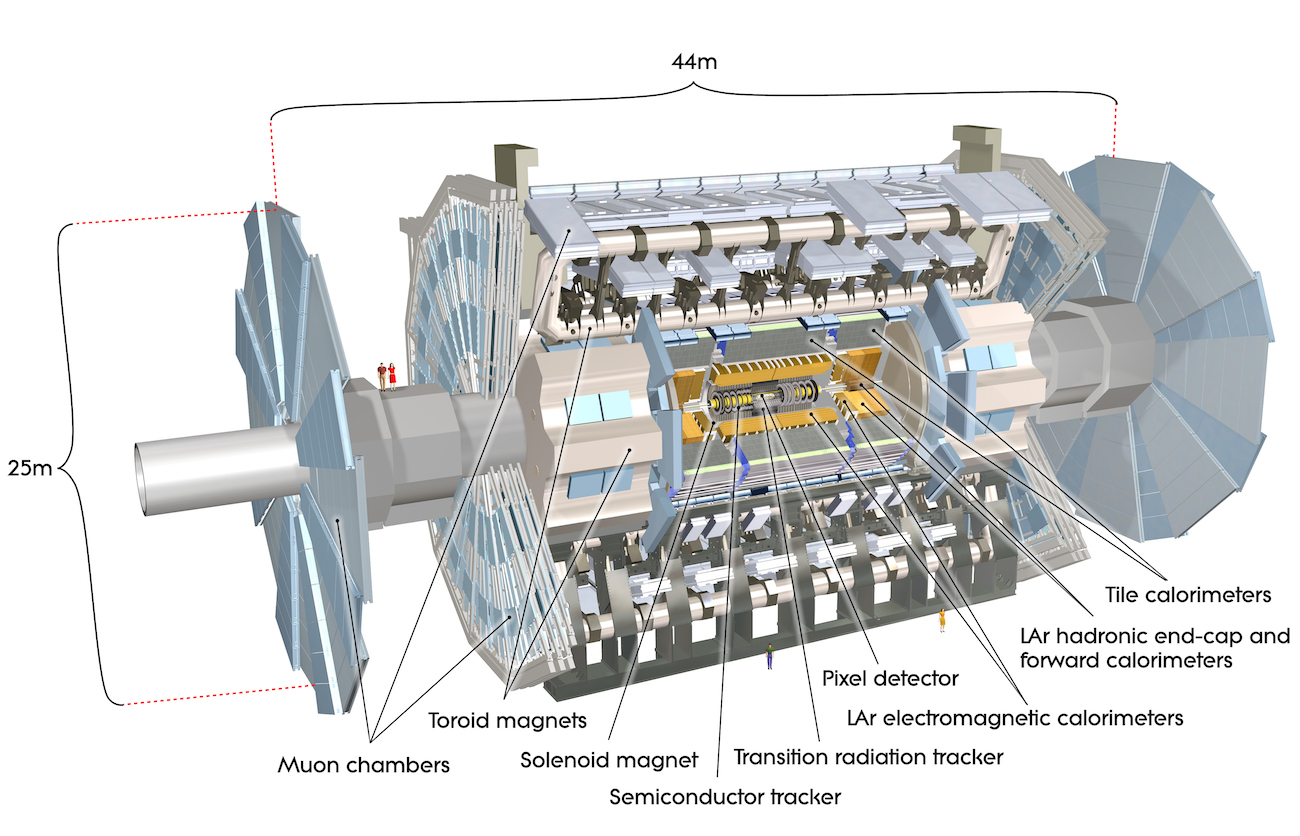
\includegraphics[width=\textwidth]{Detector/cut-away-det.jpg}
			\caption{Cut-away view of the \ac{ATLAS} detector. The dimensions of the detector are 25 m in height and 44 m in length. The overall weight of the detector is approximately 7000 tonnes~\cite{Lefevre2008}.}
			\label{fig:cut-away-det}
		\end{figure}


		\ac{ATLAS} is a general-purpose detector designed to collect data with the highest luminosity provided by the \ac{LHC}. It is located at \ac{CERN}'s Point 1 cavern and it measures about 45 m in length and 25 m in diameter. It has a forward-backward symmetric cylindrical geometry with respect to the interaction point and it is designed to reconstruct and measure physics objects such as electrons, muons, photons and hadronic jets. Its design was optimised to be as sensitive as possible to the discovery of the Higgs boson and \ac{BSM} physics. In fact, thanks to its various sub-systems, \ac{ATLAS} is able to observe all possible decay products by covering nearly $4\pi$ steradians of solid angle.

		In Figure~\ref{fig:cut-away-det} a cut-away view of \ac{ATLAS} with all its components is shown. The innermost layer is the \ac{ID} which is the core of the tracking system and consists of a Pixel, a \ac{SCT}, and a \ac{TRT}. It is submerged in a 2 T magnetic field, generated by a thin superconducting solenoid, which bends all the charged particles' trajectories allowing transverse momentum measurement. The electromagnetic and hadronic calorimeters form the next layer and they are both used to perform precise energy measurements of photons, electrons, and hadronic jets. Finally, the outermost layer corresponds to the \ac{MS}, enclosed in a toroidal magnetic field, which, together with the \ac{ID},  allows precise measurement of momentum and position of muons. These sub-detectors will be discussed in more detail in the following sections. 
	

		% --------------------------------
		% -------  THE GEOMETRY
		% --------------------------------
		\subsection*{The ATLAS coordinate system}
		\label{par:coord}
			
			A coordinate system is taken on for the spatial definition of the sub-systems %the definition of the above-mentioned physics object reconstruction, 
			and kinematic measurement of physics processes. Such system is defined starting from the interaction point, defined as the origin. The $z$-axis is defined by the beam direction and the $x-y$ plan, as transverse to the beam direction.

			A quantity, known as pseudo-rapidity, ($\eta$), is defined to describe the angle of a particle coming out of the collision, with respect to the beam axis: 

			\begin{equation*}
				\eta \equiv -\ln (\tan(\theta/2))
			\end{equation*}

			\noindent Here $\theta$ is the polar angle. The azimuthal angle, $\phi$, is defined around the beam axis and the polar angle. In the $(\eta,\phi)$ space a distance $\Delta R$ can be therefore defined as  
			
			\begin{equation*}
				\Delta R = \sqrt{{\Delta \eta}^2 + {\Delta \phi}^2}
			\end{equation*}

			\noindent where $\Delta \eta$ and $\Delta \phi$ are the differences in pseudo-rapidity and azimuthal angle between any two considered objects. A central and a forward region of pseudo-rapidity are also defined such that the detector components are described as part of the \emph{barrel} if they belong to the former or as part of the \emph{end-caps} if they belong to the latter. 



		% --------------------------------
		% -------  THE MAGNET
		% --------------------------------
		\subsection{The Magnet System}
		\label{sec:magnet-system}
			
			\begin{figure}[!htb]
				%\centering
				\subbottom[Geometry of magnet windings and tile calorimeter steel. The eight barrel toroid coils, with the end-cap coils interleaved are visible. The solenoid winding lies inside the calorimeter volume~\cite{ATLASJINST}.]{
					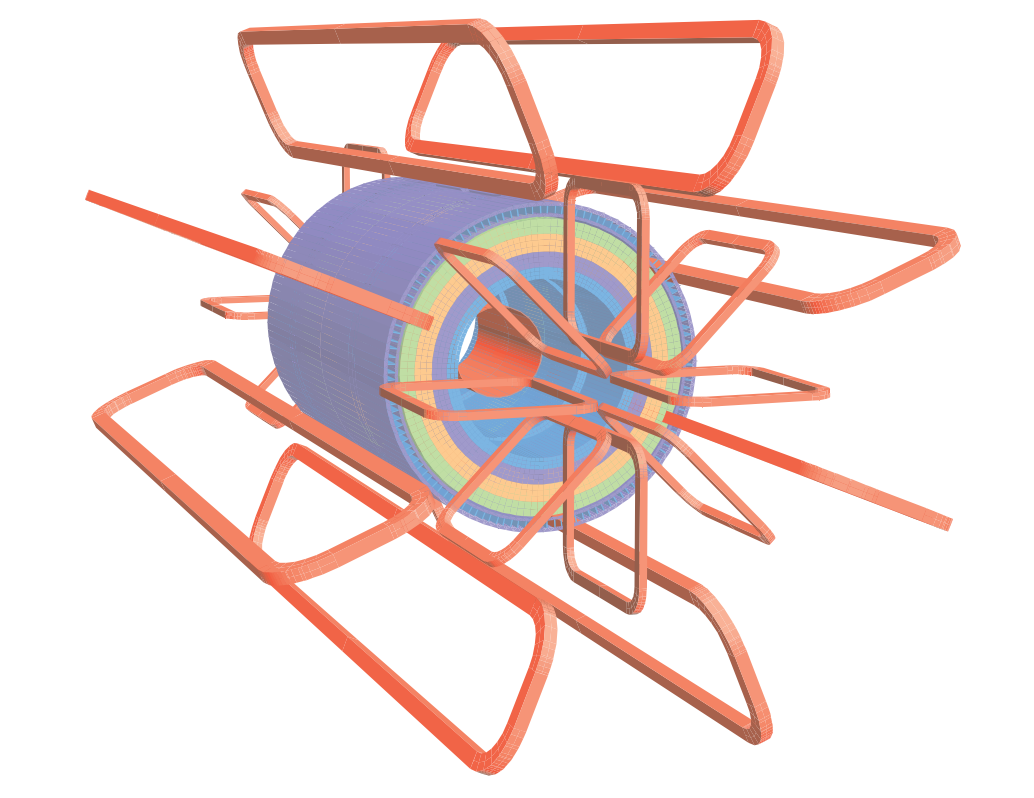
\includegraphics[width=0.475\textwidth]{Detector/MagnetSyst/magnetSyst}\label{fig:magnetSyst}}
					\hfill
				\subbottom[Schematic view of the superconducting magnets~\cite{YAMAMOTO200853}.]{
					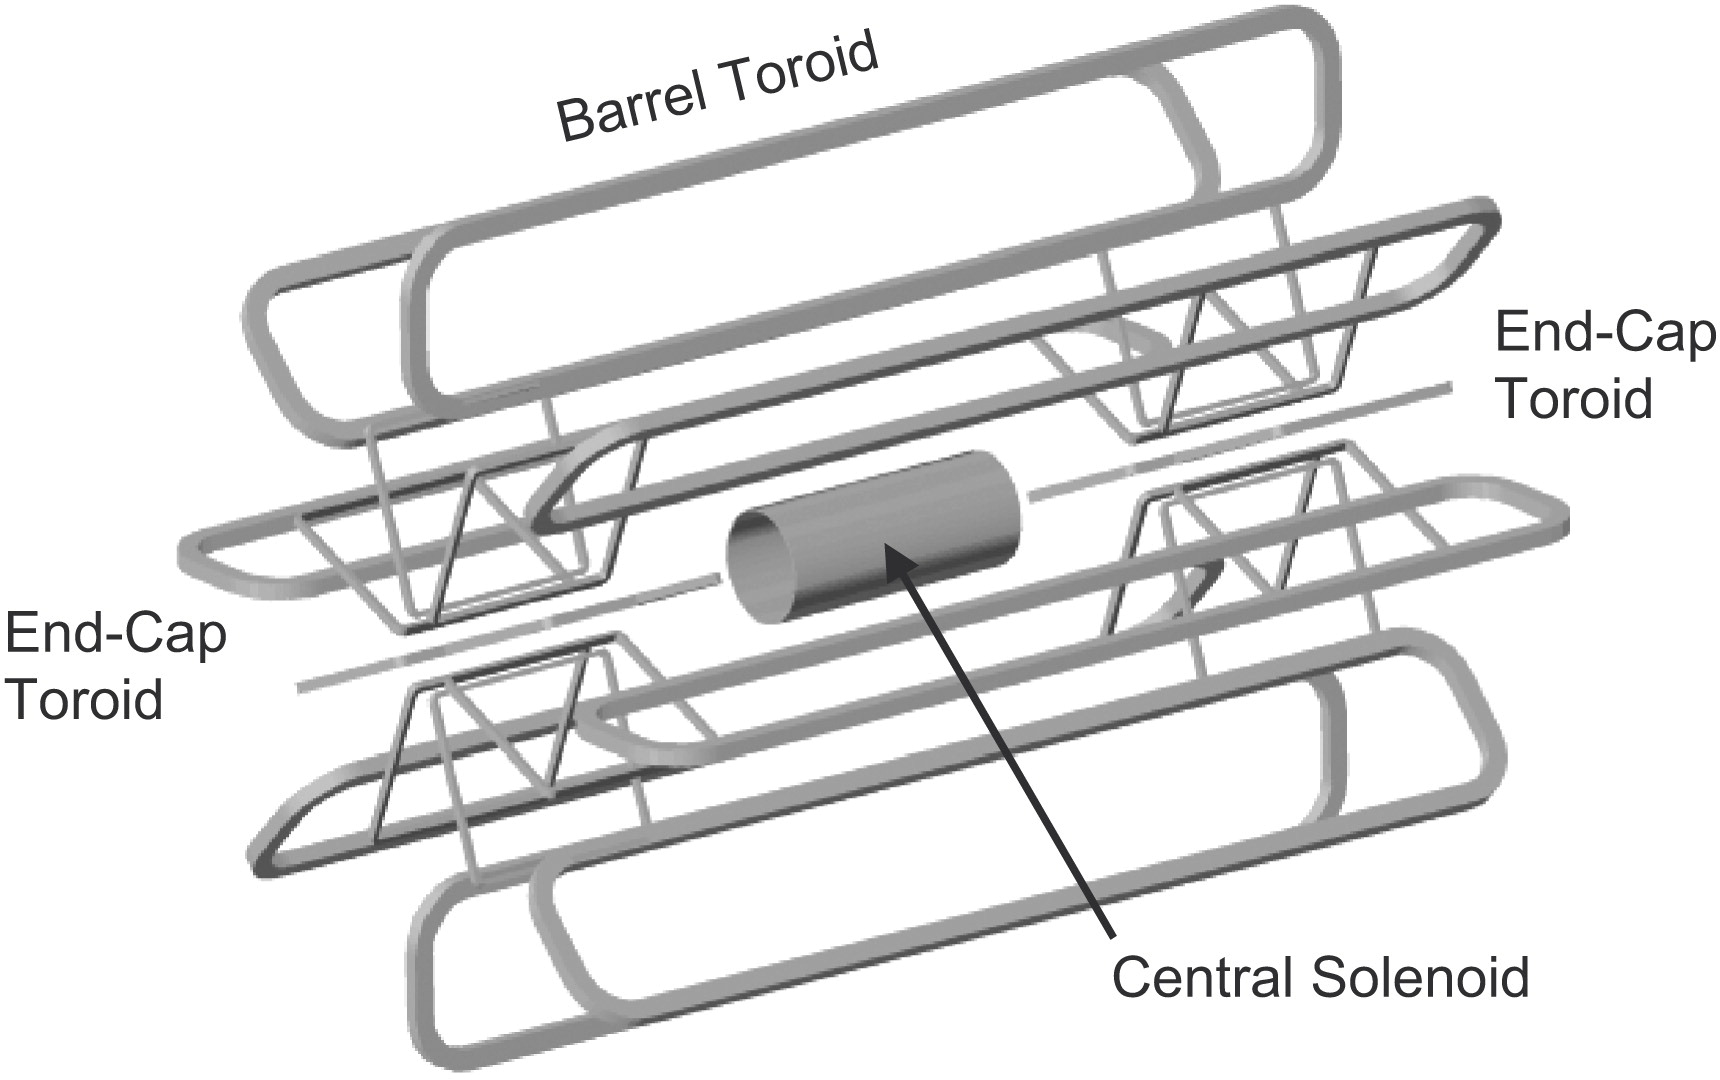
\includegraphics[width=0.475\textwidth]{Detector/MagnetSyst/magnetSyst-desc}\label{fig:magnetSyst-desc}}
				\caption{The \ac{ATLAS} magnet system.}
			\end{figure}

			\noindent The \ac{ATLAS} magnet system, 26 m long with a 22 m diameter, generates the magnetic field needed to bend the trajectories of charged particles in order to perform momentum measurement. Figure~\ref{fig:magnetSyst} and~\ref{fig:magnetSyst-desc} show the geometry of the system and its components, which are made of NbTi - superconducting material - and will be described in the following paragraphs. 



			\subsection*{The Central Solenoid}

				With an axial length of 5.8 m, an inner radius of 2.46 m, and an outer radius of 2.56 m, the central solenoid magnet is located between the \ac{ID} and the \ac{ECAL}. Its function is to bend the charged particles that go through the \ac{ID} and it is aligned on the beam axis providing a 2 T axial magnetic field that allows accurate momentum measurement up to 100 \GeV~\cite{YAMAMOTO200853}.

			\subsection*{The Barrel and the End-cap Toroids}

				Figure~\ref{fig:magnetSyst-desc} displays the toroid magnetic system that surrounds the calorimeters. With its cylindrical shape this component consists of a barrel and two end-caps toroids. The barrel toroid is comprised of eight coils and produces an approximately 0.5 T toroidal magnetic field for the central muon detectors. The end-cap toroids, also comprised of eight coils each, produce an approximately 1 T toroidal magnetic field, which is required to provide bending power for the end-cap regions of the muon spectrometer.
				
		% --------------------------------
		% -------  THE ID
		% --------------------------------
		\subsection{The Inner Detector}
		\label{sec:ID}

			The \ac{ID}~\cite{ATLASInDet} is the innermost component of the \ac{ATLAS} detector \ie\ the nearest sub-detector to the interaction region and it is used to reconstruct charged particle tracks used in the selection of physics objects. In fact, it allows robust track reconstruction, with accurate impact parameter resolution ($\sim 20 \mu m$) and precise primary and \ac{SV} reconstruction for charged particles (tracks) above 500 \MeV\ and within $\displaystyle|\eta| < 2.5$.

			\begin{figure}[!htb]
				\subbottom[Overview of the \ac{ATLAS} \ac{ID} with labels and dimensions.]{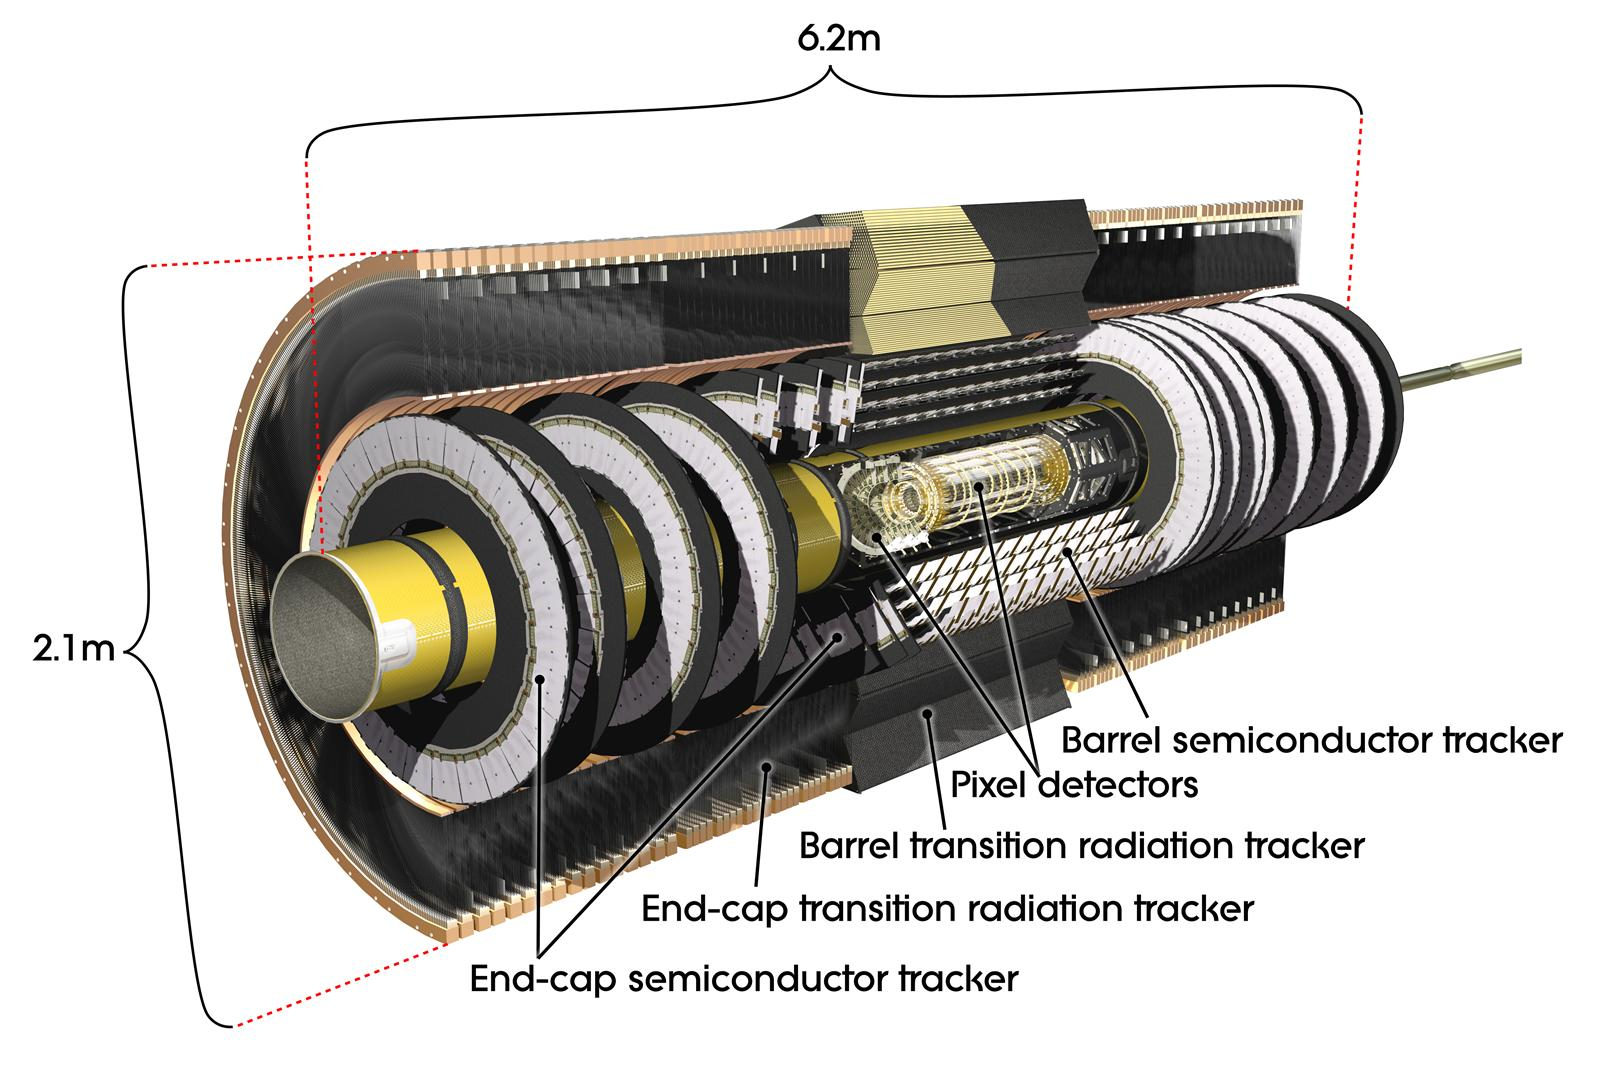
\includegraphics[width=0.475\textwidth]{Detector/ID/ID-overview}\label{fig:ID-overview}}\hfill
				\subbottom[Diagram of the \ac{ATLAS} \ac{ID} and its sub-detectors.]{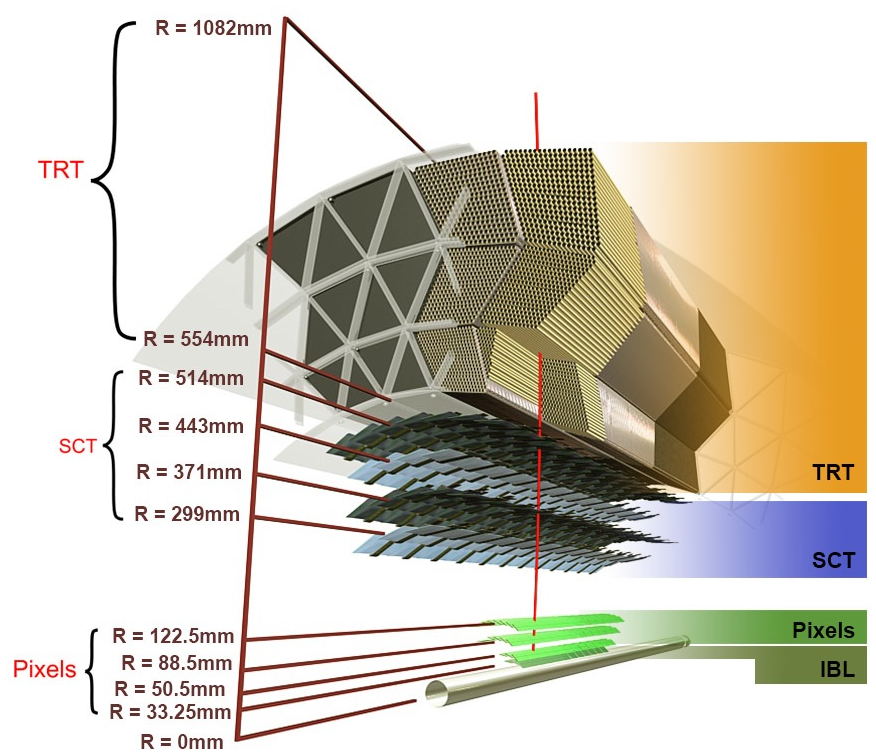
\includegraphics[width=0.475\textwidth]{Detector/ID/ID}\label{fig:ID}}
				\caption{The \ac{ATLAS} Inner Detector}
				\label{fig:AID}
			\end{figure}


			The \ac{ID} is comprised of independent and concentric sub-systems, which are all shown in Figure~\ref{fig:AID}: %\ref{fig:ID} and~\ref{fig:ID-overview}:

			\begin{description}
				\item \textbf{\ac{IBL}:} \\innermost Pixel Detector layer added during \ac{ATLAS} Run 2 upgrade (2013/2014) to improve vertexing, by a factor $\sim 1.4$, and impact parameter reconstruction, by a factor 2;
				\item \textbf{Silicon Pixel Tracker (Pixel):} \\made of silicon pixel layers and used mainly for reconstructing both the primary and secondary vertices in an event;
				\item \textbf{\ac{SCT}:} \\comprised of silicon micro-strip layers; thanks to its resolution ($17 \times 580\, \mu$m) it can accurately measure particle momenta;
				\item \textbf{\ac{TRT}:} \\final layer comprised of various layers of gaseous straw tube elements surrounded by transition radiation material.
			\end{description}

			These sub-detectors will be discussed in the following sections.  

			\subsection*{IBL} 
				
				The \ac{IBL}~\cite{IBLTDR} is the innermost Pixel Detector layer as shown in Figure~\ref{fig:ID}. It is comprised of 6M channels and each pixel measures $50 \times 250\,\mu$m. Its resolution is $8 \times 40\, \mu$m. The addition of this new layer produced an improvement on the quality of the impact parameter reconstruction of tracks almost by a factor 2, and almost by a factor 1.4 on the resolution of the reconstructed \ac{PV}, highly important \eg\ for the tagging of bottom-quark-initiated jets (\emph{b}-jets). %which, in case of a B-layer failure, can be restored by the \ac{IBL}. Besides these improvements, the \ac{IBL} insertion allowed \ac{ATLAS} to better cope with high luminosity effects such as the increase in event pile-up, which leads to high occupancy and read-out inefficiency. 

			\subsection*{Pixel}
				
				The Pixel detector is comprised of 1750 identical sensorchip-hybrid modules, each covering an active area of 16.4 $\times$ 60.8 mm. The total number of modules correspond to roughly 80 million semiconductor silicon pixels. The nominal pixel size is 50 $\mu$m in the $\phi$ direction and 400 $\mu$m in the barrel region, along the $z$-axis (beam axis)~\cite{ATLASPix}. The reason why such a large amount of pixels is employed is justified by the need to cope with the high luminosity in \ac{ATLAS}. The silicon pixel detector measures 48.4 cm in diameter and 6.2 m in length providing a pseudo-rapidity coverage of $\abseta < 2.5$. Figure~\ref{fig:ID} shows the three concentric barrel layers placed at 50.5 mm, 88.5 mm and 122.5 mm respectively. Furthermore, the Pixel detector is made of six disk layers, three for each forward region, such that when a charged particle crosses the layers it will generate a signal at least in three space points. The fine granularity of such detector allows accurate measurement and precise vertex reconstruction, as it provides a more accurate position measurement as a large detection area is available. In particular, it has a resolution of $10 \times 115\,\mu$m.

			\subsection*{SCT}

				The \ac{SCT} is made of 4088 modules of silicon micro-strip detectors arranged in four concentric barrel layers. It is mainly used for precise momentum reconstruction over a range $\abseta < 2.5$ and it was designed for precision measurement of the position using four points (corresponding to eight silicon layers), obtained as track hits when crossing the layers. Figure~\ref{fig:ID} shows the structure of the \ac{SCT} with its four concentric barrel layers with radii ranging from 299 mm to 514 mm and two end-cap layers. Each module has an intrinsic resolution of 17 $\mu$m in the $R-\phi$ direction and 580 $\mu$m in the $z$ direction. As the \ac{SCT} is further away from the beam-pipe than the Pixel detector, it has to cope with reduced particle density. This allows for reduced granularity maintaining the same level of performance of the Pixel detector: \ac{SCT} can use $\sim$ 6.3 million read-out channels.%, almost 2 million fewer than the pixel detector.


			\subsection*{TRT}
			 
				The last and outermost of the sub-systems in the \ac{ID} is the \ac{TRT}. It is a gaseous detector which consists of 4 mm diameter straw tubes wound from a multilayer film reinforced with carbon fibres and containing a 30 $\mu$m gold plated tungsten wire in the centre. The straw is filled with a gas mixture of 70\% Xe, 27\% CO$_2$ and 3\% O$_2$~\cite{TRT2012}. As shown in Figure~\ref{fig:ID}, its section consists of three concentric layers with radii ranging from 554 mm to 1082 mm, each of which has 32 modules containing approximately 50,000 straws, 1.44 m in length, aligned parallel to the beam direction with independent read-out at both ends. The gas is ionised when a charged particle passes through it and electrons (ions) are collected at the anode (cathode). A current in the wire will be created and as the electric field in the tube is known, the distance from the wire can be calculated using the time that electrons take to drift to the wire. 
				Furthermore, the \ac{TRT} is capable of performing particle identification on the particles that pass through it by utilising the detection of transition radiation photons that are emitted when a highly relativistic charged particle crosses a boundary between two media with different dielectric constants. The separation between, \eg\ electrons and charged pions is achieved by observing the amount of transition radiation produced, since this is dependent on how relativistic the charged particle is.

				The \ac{TRT} has an intrinsic resolution of 130 $\mu$m and, on average, 35 hits are observed within such sub-system when a charged particle passes through.

				%Both end-cap sections are divided into 14 wheels, with roughly 320,000 straws in the R-direction. The average 36 hits per track in the central region of the \ac{TRT} allow continuous tracking to enhance pattern recognition and momentum resolution in the $\left| \eta \right| < 2.5$ region. %It also improves the \pt\ resolution for longer tracks.

			\subsection*{Performance of the ID}

				As previously mentioned, the tracking performed by the \ac{ID} is indispensable to measure the properties of objects such as leptons and jets, as well as interaction vertices in a certain event and secondary vertices, which are used \eg\ to identify bottom-quark-initiated jets(\bjs). Both jets and \bjs\ are expected in the final states that are being searched for in this thesis. 

				The overall performance of the \ac{ID} depends on the three sub-systems and it can be shown in terms of momentum resolution: 

				\begin{equation}
				\label{eq:IDperf}
					\displaystyle \frac{\sigma_{\pt}}{\pt} = 1.6 \pm 0.1\% \oplus \frac{(53 \pm 2) \times 10^{-5}}{\GeV} \times \pt
				\end{equation}

				\noindent measured in~\cite{Aad2011} using cosmic muons before the addition of the \ac{IBL}. Eq.~\ref{eq:IDperf} shows that the \ac{ID} has a momentum resolution of $\sim 1.6\%$ at low momenta ($\sim 1 \GeV$) and of $\sim 50\%$ at $1$ TeV.

		% --------------------------------
		% -------  THE CALORIMETERS
		% --------------------------------
		\subsection{The Calorimeters}

			\begin{figure}[!htb]
				\centering
				\includegraphics[width=\textwidth]{Detector/Calo/Calo-overview}
				\caption{A computer generated image of the full calorimeter.}
				\label{fig:Calo}
			\end{figure}

			The \ac{ATLAS} Calorimeter system, shown in Figure~\ref{fig:Calo}, is comprised of two main sub-systems; the \ac{ECAL} and \ac{HCAL}, which are designed to stop and measure the energy of electromagnetic-interacting and hadronic particles respectively. The combination of the two provides full coverage in $\phi$ and $\abseta < 4.95$. Particles slow down and lose energy generating showers when crossing different layers. The \ac{ECAL} is comprised of one barrel and two end-cap sectors employing \ac{LAr}. The showers hereby develop as electrons pairs which are then collected. The \ac{HCAL} is also comprised of one barrel and two end-cap sectors. The sensors in the barrel of the \ac{HCAL} are tiles of scintillating plastic whereas \ac{LAr} is employed for the end-cap. A forward region, the closest possible to the beam, is covered by a \ac{LAr} forward calorimeter (FCal). The \ac{LAr} and Tile Calorimeter will be briefly discussed in the following paragraphs. 
			%The particles have to deposit all their energy within the calorimeters to obtain an accurate energy measurement and avoid energy deposits in the outer muon spectrometer.
			%The definitions of radiation length ($X_0$), the distance over which an electron loses 1/$e$ of its energy within a given material, and nuclear interaction length ($\lambda_I$), are used to define the lengths of the barrel and the endcap regions of the calorimeter system. The \ac{ECAL} roughly measures 22 $X_0$ thick in the region of barrel, and 24 $X_0$ in the end caps. The \ac{HCAL} roughly measures 10 $\lambda_I$. Both \ac{ECAL} and \ac{HCAL} measures vary with $\eta$. Furthermore, it is known that hadronic particles are more penetrating than the electromagnetic ones and in particular, $\lambda_I$ is roughly ten times bigger than $X_0$. 

			\subsection*{The Liquid Argon Calorimeter}

 				The \ac{ECAL} is comprised of multiple layers of \ac{LAr} sampler and lead absorber. The choice of its accordion-geometry design brought two main advantages; full $\phi$ coverage with no non-interactive regions (no cracks); fast extraction of signals coming from both front or rear end of the electrodes. It is made of two half-barrel wheels, both placed in the barrel cryostat, that provide a pseudo-rapidity coverage up to $\left | \eta\right | < 1.475$ and two end-cap detectors providing $1.375 \leq \abseta \leq 3.20$ coverage in two end-cap cryostats. The junction between the barrel and end cap components defines the crack region and any signal coming from the crack region is therefore discarded. 

 				In the $\left | \eta\right | < 1.8$ region there is an additional layer, placed at the front of the calorimeter, that is made of a thin (0.5 cm in the end-cap and 1.1 cm in the barrel) \ac{LAr} layer with no absorber~\cite{ATLASLAR}. This additional layer was designed to correct for the energy lost, as particles enter the calorimeter, by taking a measurement just before the majority of the electromagnetic shower is developed. 

 				%Two separate readout paths are employed: one with coarse granularity (\emph{trigger towers}), and one with fine granularity. These which will be further discussed in Chapter \ref{ch:trigger}.

 				% In the barrel, the accordion layers are axial and run in $\phi$, the folding angles of the layers vary with radius to keep the liquid-argon gap constant. 
 				% In the end-caps the layers are parallel to the radial direction and run axially. 
 				% The \ac{LAr} is ionised by electromagnetic showers. The read-out circuits are made of three copper layers insulated by two layers of polyimide. 
 				% The two outer layers, split in sectors, are connected to high-voltage sources and polarize the \ac{LAr} gap to the absorber. 
 				% The inner layer is where the signal is collected through capacitive coupling and is then segmented into read-out pads.

			\subsection*{The Tile calorimeter}

				The main purpose of the hadronic calorimeter is to measure the energy of hadronic showers. It is built employing steel and scintillating tiles coupled to optical fibres which are read out by photo-multipliers. As shown in Figure~\ref{fig:Calo}, the \ac{HCAL} is made up of three cylinders; a central barrel, 5.64 m long covering a region $\abseta < 1.0$, and two extended barrel, 2.91 m long covering a region $0.8 < \abseta < 1.7$. Each cylinder is made up of 64 modules and each module is in turn made up of three layers. Ultimately, the smallest section of the calorimeter module is a cell with a $\Delta \phi \times \Delta \eta = 0.1 \times 0.1$ granularity for the two innermost layers and $\Delta \phi \times \Delta \eta = 0.2 \times 0.1$ for the outermost one. 

			\subsection*{Performance of the Calorimeter}

				The performance of the calorimeter is important to measure the properties of the jets used in the analyses presented in this thesis. This has been assessed using test beam data and, once the noise has been subtracted from the experimental measurements these are fit using Eq.~\ref{eq:caloPerf}

				\begin{equation}
				\label{eq:caloPerf}
					\frac{\sigma(E)}{E} = \frac{a}{\sqrt{E [ \GeV ] }} \oplus b
				\end{equation}

				\noindent Here, $a$ is the stochastic term and $b$ is a constant that includes local non-uniformities in the calorimeter response. 

				The \ac{ECAL} performance in the barrel was assessed firing an electron beam at a module that is identical to those in \ac{ATLAS} and the fitted energy resolution is $\sigma(E)/E = (10 \pm 0.4)\% / \sqrt{E} \oplus (0.4 \pm 0.1)\%$ with a variation of no more than 0.7\% for the entire coverage of the calorimeter.

				The \ac{HCAL} performance in the barrel was assessed firing a pion beam at a prototype detectors of the \ac{LAr} electromagnetic and tile calorimeters. The fitted energy resolution (with an added term to account for electronic noise) is $\sigma(E) / E = (52 \pm 1.0)\% / \sqrt{E} \oplus (3.0 \pm 0.1)\% \oplus (1.6 \pm 0.1) / E$. 


		% --------------------------------
		% -------  THE MU SPEC
		% --------------------------------
		\subsection{The Muon Spectrometer}
		\label{sec:MuSpec}

			The \ac{MS}~\cite{MSTDR}, shown in Figure~\ref{fig:MS}, is the outermost sub-system of the whole \ac{ATLAS} detector. As such, it surrounds the calorimeters and its main function is to perform precision measurement of muons momenta. The deflection of muon tracks employing large superconducting air-core toroid magnets and high-precision tracking chambers is at the heart of such high precision measurement. 

			\begin{figure}[!htb]
				\centering
				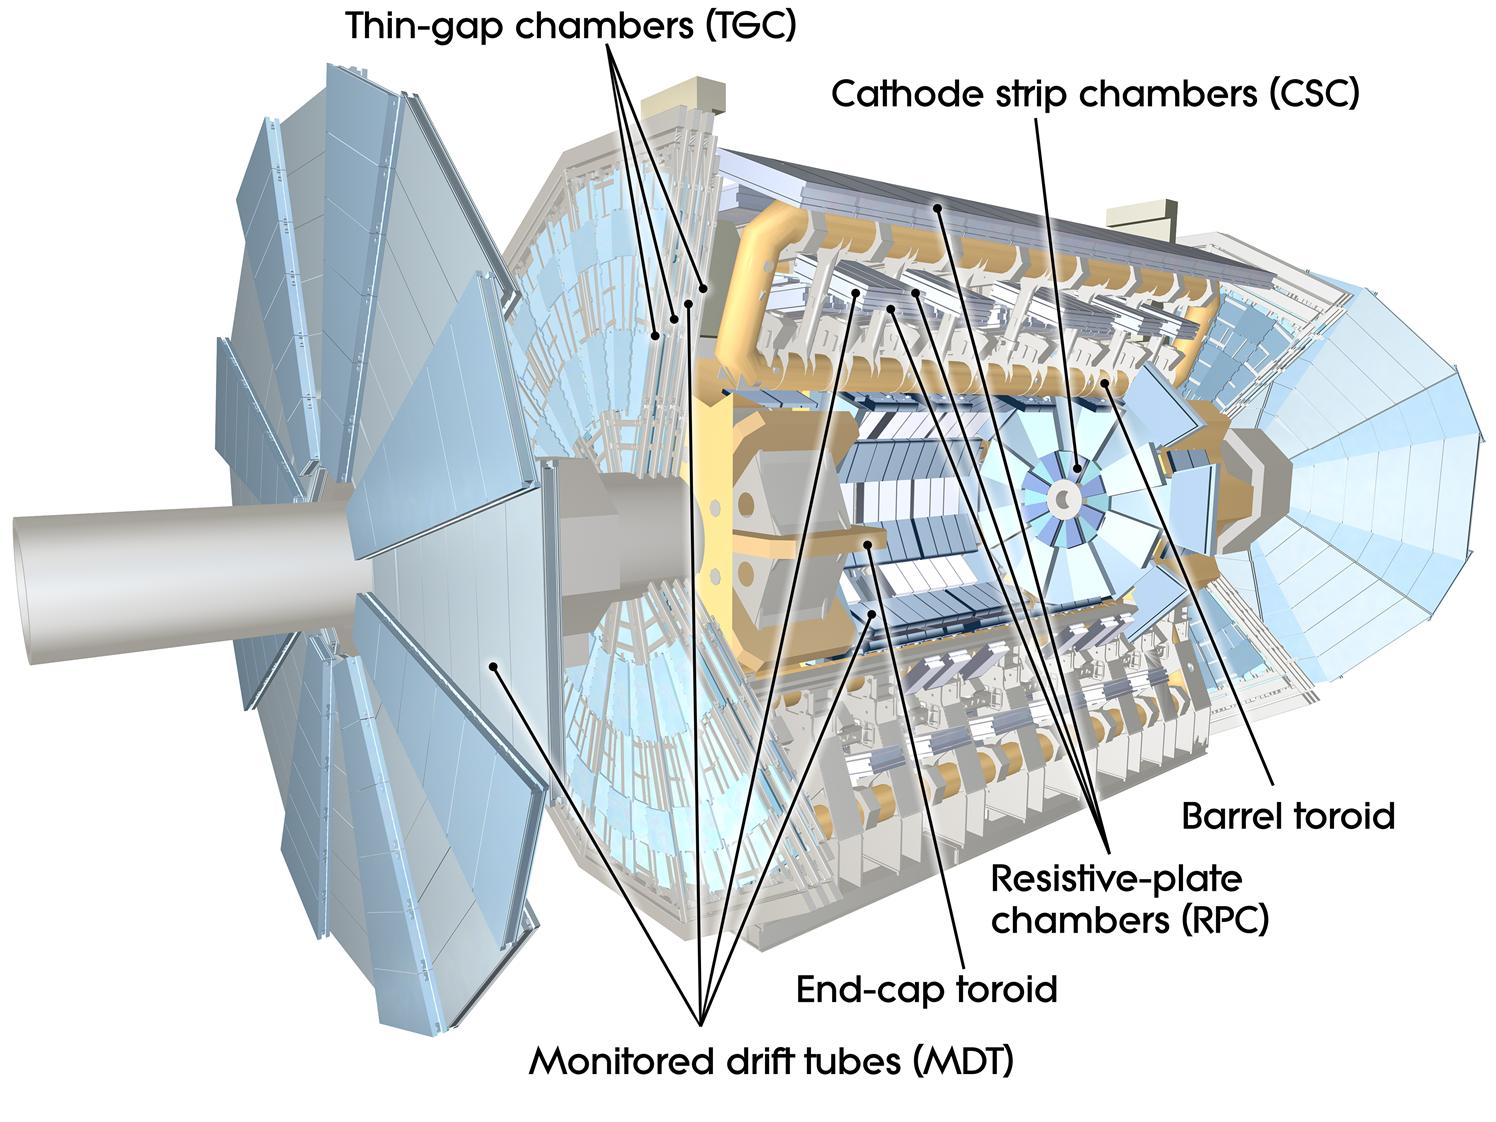
\includegraphics[width=\textwidth]{Detector/MS/MS}
				\caption{Cut-away view of the \ac{ATLAS} muon system~\cite{ATLASJINST}.}
				\label{fig:MS}
			\end{figure}

			The \ac{MS} is comprised of one large barrel toroid, covering the region $\left| \eta \right | \leq 1.4$, and two end-cap toroids, covering $1.6 < \left| \eta \right| \leq 2.7$ which are employed together to achieve the track-bending effect wanted. The magnitude of the magnetic field in the barrel, generated by eight large superconducting coils, ranges from 0.5 to 2 T. 

			Around the beam axis, three cylindrical layers make way for the chambers, placed in planes perpendicular to the beam, used to measure tracks. 

			\acp{MDT} are employed over most of the pseudo-rapidity range to provide precision measurement of track coordinates in the bending direction. An MDT is essentially a set of 30-mm-diameter Aluminium tubes containing a \emph{W-Re} (Tungsten-Rhenium) wire, surrounded by a non-flammable $\mathrm{Ar}$-$\mathrm{CH_4}$-$\mathrm{N_2}$ mixture at a pressure of 3 bar. The resolution a single wire can give on the particle position is 80 $\mu$m enhanced by having multiple layers of tubes for each module.
			
			\acp{CSC} are instead employed at large pseudo-rapidity ($2 < \abseta < 2.7$). They work similarly to the MDT but instead of tubes there are cathode strips above and below the anode wires. In particular, one set is orthogonal to the wires for precision measurement and the other one parallel to the wires providing a measurement of the transverse coordinate. The gas employed between the strips and wires is a non-flammable mixture of $\mathrm{Ar}$-$\mathrm{CO_2}$-$\mathrm{CF_2}$.

			\acp{TGC} are employed in the end-cap region and \acp{RPC} in the barrel. The \acp{TGC} are very similar to the \acp{CSC}. They provide large signals and in a very narrow time window making them ideal for triggering purposes.

			The \acp{RPC} are also gas-based detectors. They are comprised of two parallel resistive plates held apart by insulating spacers, and a uniform electric field is employed to generate a limited avalanche multiplication centred around the primary ionisation electron. This will then be detected by \emph{Al} strips separated from the plates by an insulating film.

			%\acp{TGC} and \acp{RPC} will be mentioned again in ~\ref{sec:L1} as they are part of the trigger system.



	% --------------------------------
	% -------  THE TRIGGER
	% --------------------------------
	\section{The ATLAS Trigger System}
	\label{sec:trigSyst}

		The \ac{ATLAS} Trigger System is at the heart of data taking. It is an essential component of any nuclear or particle physics experiment as it is responsible for deciding whether or not to store an event for later study. Its main function to reduce the event rate from $\sim$ 40 MHz bunch-crossing\footnote{The term bunch-crossing, \mubar, is hereby used when referring to a collision between two bunches of protons.} to $\sim 1$ kHz.

		The Trigger system employs a two-level system: a first hardware-based trigger, \ac{L1} Trigger, and a software-based, \ac{HLT}. \ac{L1} processes low-granularity information from the calorimeter and the muon spectrometer and identifies the so-called Regions of Interest (RoIs)\footnote{$\eta - \phi$ regions where event features have been found by the \ac{L1} selection process.} before making a decision. Event data from other sub-system are temporarily stored in memories whilst \ac{L1} decision is taken.
		
		Further investigations are left to \ac{HLT} which is made of software running on a cluster of computers (\ac{HLT} farm). Additionally, a \ac{FTK} system~\cite{FTKTDR} (to be installed before the end of Run 2) will process events that are accepted by \ac{L1} trigger, and seed the \ac{HLT} algorithms. It will provide global \ac{ID} track reconstruction at the \ac{L1} trigger rate using lookup tables stored in custom associative memory chips for the pattern recognition.
		
		The \ac{ATLAS} trigger system will be further discussed in Chapter~\ref{ch:trigger}, however the Run-1-to-Run-2 upgrade of the \ac{ATLAS} trigger will not be discussed any further.